%!TEX root = main.tex

\subsection{\textbf{RQ3:} How well do tools support developer's needs for managing merge conflicts?}\label{RQ3}

Development tools need to be easy to use and provide contextualized, pertinent information in a manner that is easy to understand.
To investigate how well current tools satisfy the needs of developers, we asked interview participants open-ended questions about how they resolve merge conflicts.
We also ask about improvements that would be most valuable to them.

We framed the S2 survey questions to validate the improvement needs expressed in our interviews, and ranked those six needs according to mean score.
Table~\ref{s2_tool_improvements} presents the needs from the S2 survey responses ordered by their mean scores.
We received 119 responses using a 5-point Likert-type scale to indicate the usefulness of each type of tool improvement (1 being \textit{Not Useful}, 3 being \textit{Moderately Useful}, and 5 being \textit{Essential}).

\begin{table}[!htbp]
\renewcommand{\arraystretch}{1.2}
\caption{Desired Improvements to Merge Toolsets from Barriers Survey (S2)}
\label{s2_tool_improvements}
\centering
\begin{tabularx}{\textwidth}{>{\rowmac}c | >{\rowmac}l | *1{>{\rowmac}c} | *2{>{\rowmac}c}<{\clearrow}}
\toprule
  \parnoteclear % tabularx will otherwise add each note thrice
  Imp.\parnote{Imp. = Improvement} & Description & \likertscale{1,2,3,4,5} & Median\parnote{Responses on 5-point Likert scale indicating the degree of potential impact on merge conflict processes (1 indicates \textit{no impact}, 5 indicates \textit{great impact}).\vspace*{-0.3\baselineskip}} & Mean\textsuperscript{ii} \\
\midrule
  I1 & Usability & \likertplot{coordinates {(1,6)(2,17)(3,32)(4,48)(5,16)}}{28.2}{6,17,32,48,16} & 4 & 3.43 \\
  I2 & Filtering of relevant information & \likertplot{coordinates {(1,8)(2,15)(3,32)(4,48)(5,16)}}{28.2}{8,15,32,48,16} & 4 & 3.41 \\
  I3 & Support for exploring project history & \likertplot{coordinates {(1,7)(2,21)(3,36)(4,39)(5,16)}}{28.2}{7,21,36,39,16} & 3 & 3.30 \\
  I4 & Graphical information presentation & \likertplot{coordinates {(1,13)(2,26)(3,26)(4,37)(5,16)}}{28.2}{13,26,26,37,16} & 3 & 3.14 \\
  I5 & Transparent tool functionality/operations & \likertplot{coordinates {(1,16)(2,36)(3,24)(4,40)(5,3)}}{28.2}{16,36,24,40,3} & 3 & 2.82 \\
  I6 & Terminology consistent with other tools\hspace{0.5cm} & \likertplot{coordinates {(1,23)(2,41)(3,32)(4,15)(5,8)}}{28.2}{23,41,32,15,8} & 2 & 2.53 \\
\bottomrule
\end{tabularx}
  \parnotes
\end{table}

Our results indicate that developers use a wide range of tools, with many directly using the Git command line interface. 
Our interview participants mentioned six different dimensions along which they would like improvements to tool support.

In addition, we also asked S2 survey participants which tools they use during conflict resolution.
We identified 105 different tools from the 115 responses. 
Some mentioned generic responses such as \textit{``text editor''}, for which we create a separate category.
%We group these generic responses together where semantically similar meanings exist. 
Table~\ref{s2_toolset} lists the top 10 most common tools used by participants to resolve merge conflicts.

\begin{table}[!htbp]
\renewcommand{\arraystretch}{1.3}
\caption{Merge Resolution Toolsets (Top 10) from Barriers Survey (S2)}
\label{s2_toolset}
\centering
\begin{tabularx}{\textwidth}{ll|c}
\toprule
  \parnoteclear % tabularx will otherwise add each note thrice
  Tool & Description & \# Participants (\%)\parnote{
  Survey participants were allowed to provide multiple tools. Each entry represents the number (and percentage) of participants that responded with that particular tool. 115 out of 162 respondents (70.99\%) indicated the use of at least one merge resolution tool.\vspace*{-0.3\baselineskip}}\\
\midrule
  Git & Version Control System & 37 (15.68\%)\\
  Vim/vi & Text Editor & 17 (7.20\%)\\
  Text Editor (unspecified) & Text Editor & 14 (5.93\%)\\
  Git Diff & Diffing Tool & 11 (4.66\%)\\
  GitHub & Website & 11 (4.66\%)\\
  Eclipse & IDE & 10 (4.24\%)\\
  KDiff3 & Diff \& Merge & 9 (3.81\%)\\
  Meld & Diff \& Merge & 8 (3.39\%)\\
  SourceTree & Git/Hg Desktop Client & 8 (3.39\%)\\
  Sublime Text & Text Editor\hspace{3.2cm} & 7 (2.97\%)\\
\bottomrule
\end{tabularx}
\parnotes
\end{table}

In examining the list of these tools, we note that developers most often use basic tools (e.g. Git, Vim/vi, or a Text Editor) to handle merge conflicts instead of employing specialized tools or plugins to modern IDEs. 
In this list, there is only one IDE (Eclipse), and three diff/merge toolsets (Git Diff, KDiff3, and Meld). 
Along with the list of toolsets used for evaluating whether a merge resolution was successful (see Table~\ref{resolution-evaluation-tools}), we find that developers lack proactive conflict detection tools and code analysis tools that could address many of the developer needs (see Table~\ref{s2_needs}) and desired improvements (see Table~\ref{s2_tool_improvements}).

We next discuss the top four improvements rated by survey respondents. These are the responses that have a mean value higher than $3.00$.

\nsubsection{Better Usability}
%The right toolset is essential for efficiently developing solutions and resolving conflicts.
Usability is an important factor that determines whether a toolset supports or hinders the developer's workflow.
Our S2 survey results indicate that \textit{better usability} (I1) is the most desired improvement of toolsets used for conflict resolution. 
%Based on the results of the survey, we found that practitioners rate usability as the most desired improvement for their current merge tools (I1).
While usability of a particular tool is important, the usability concerns become even more pertinent when they span multiple tools that are similar and must operate in sync with each other.
Survey results indicate that participants use an average of 2.5 tools, and as many as 7 tools, to resolve merge conflicts.
%With multiple tools being used during merging and conflict resolution, toolset fragmentation is a real concern for practitioners.
For instance, in our interview P1 demonstrated how he typically resolved a merge conflict by using four different tools and said: 
\begin{quoting}
\textit{``I have to jump around between tools and copy and paste version numbers...this is why integration matters.''}
\end{quoting}

Switching across multiple tools while resolving a conflict is disruptive and comes at a cost. 
Psychology studies~\cite{Meiran2000}\cite{gopher2000switching} have shown that task switching reduces performance and causes mental fatigue. 
Gerald Weinberg highlighted that context switching arising from toolset fragmentation is a big problem in engineering teams~\cite{Weinberg1992}. 

%This frustration is understandable for practitioners whose workflows frequently get interrupted by tool switches. Psychology studies~\cite{Meiran2000}\cite{gopher2000switching} have found that task switching comes with costs in performance and mental fatigue, and, in 1992, Gerald Weinberg highlighted the problem of toolset fragmentation within engineering teams~\cite{Weinberg1992}. 

\nsubsection{Better Exploration of Project History}
Developers have been known to use historical data to understand code evolution and development processes~\cite{Mihai_lenses}.
Version control and bug tracking systems contain a huge amount of meta-information about the evolution of code and development processes.
However, it is not easy to find the right bit of information in these large systems. 
Currently, there is insufficient support for performing detailed analysis of how a code snippet evolved over time and why. 
Better ways of exploring the project history (I3) was one of the top requested improvements in our survey. 
As P1 mentioned in the interview:
\begin{quoting}
\textit{``Give me a way to explore the history. To drill down, to go back up, you know? To resurface and understand what happened.''}
\end{quoting}


Currently, when performing any complex analysis it is easier to write stand alone scripts to extract the information. 
During the interview, P1 mentioned that he has written several scripts to locate particular historical commits that relate to a current merge conflict. 
Similarly, P9 described a tool, \texttt{git-diff}, that was developed by their team to add additional difference analysis functionality across branches:
\begin{quoting}
\textit{``git-diff will just do the diff based on the SHAs... we're adding metadata... It also hooks into GitHub labels to do some more advanced heuristics.''}
\end{quoting}

While writing these scripts allows extraction of relevant data contextualized to the need, it also leads to a proliferation of multiple scripts that are written by individual developers and need to be maintained or integrated.
This further adds to the problem of context-switching when developers must switch between multiple tools, and execute multiple scripts.

We are not the first to recognize the gap in tool support provided for analyzing development history among developers~\cite{Mihai_lenses, sun2015informationhistory, guo2016cold-start, yan2014miningcontracts}. 
It appears that practical applications of history exploration are still beyond the reach of developers. 
One of the reasons for this might be the simple set of text editors, and toolsets, that our study participants seem to prefer.

\nsubsection{Better Filtering of Less-Relevant Information}\label{better_filtering}
Tools that routinely handle large or complex datasets require filtering in order to efficiently locate desired pieces of information.
For example, when there are several commits in a pull request and multiple levels of code review at the line level.
It is difficult to extract the key issue in the pull request, which can get lost in the sea of low level details. Similarly, if there are multiple commits in a pull request or branch, it is hard to extract the right information.
Therefore, tools that provide filtering can better assist developers in working with large amounts of metadata associated with the changes.
\textit{Better ways of filtering out less relevant information} (I2) was selected as the second most important need; P1 explained:
\begin{quoting}
\textit{``You want to extract the relevant commits. The ones that actually clash...you want to zoom in on them and understand just enough and don't waste time.''}
\end{quoting}

While improvements in history exploration (I3) will make project metadata more accessible, improvements in filtering for relevant metadata will allow developers to focus on the relevant parts of the code impacted by the merge conflict.

%Version control systems (VCS) and bug tracking systems provide insufficient support for detailed analysis of software evolution and information retrieval~\cite{fischer2003release_history}.
%For software practitioners using \texttt{git} and other VCS, it is often easier to write scripts that accommodate their particular information needs by augmenting the capabilities of the VCS.
%During the interviews, P1 described writing several scripts in order to locate particular historical commits that relate to a current merge conflict.
%P9 also described a tool, \texttt{git-diff}, developed as part of their efforts to add additional difference analysis functionality across branches:
%\begin{displayquote}
%\textit{``git-diff will just do the diff based on the SHAs... we're adding metadata and cherry picking, so the SHAs are always going to be changing... It also hooks into GitHub labels and uses the labels on the project to do some more advanced heuristics.''}
%\end{displayquote}
%\todo{Shane: This transition is a bit rough}
%In our survey results, we see that practitioners rank \textit{better ways of filtering out less relevant information} (I2) as the second highest improvement needed in modern merge toolsets.
%This suggests that further work is needed to bring these capabilities from single-purpose scripts into common toolsets used by all practitioners.
%
%\Subsubsection{Better Exploration of Project History}
%Codoban et al.~\cite{mihai_lenses} introduced the concept of the \textit{Archeology Lens} to describe examining old development history to retrieve lost knowledge and postulated that additional tool support was needed in this context.
%We also find that practitioners consider history exploration to be a major area of improvement for development toolsets.
%Among survey participants, \textit{better ways of exploring project history} (I3) ranked as the third most important improvement needed.
%During our interviews, P1 said: 
%
%\begin{displayquote}
%\textit{``Give me a way to explore the history. To drill down, to go back up, you know? To resurface and understand what happened.''}
%\end{displayquote}
%
%The gap in support for analyzing development history among practitioner toolsets has previously been recognized by researchers~\cite{sun2015informationhistory, guo2016cold-start, yan2014miningcontracts}, however practical application of these efforts appear to have not yet reached practitioners.

\nsubsection{Better Graphical Presentation of Information}
The usefulness of information is helped or hindered by the way in which it is presented to users.
In our survey results, we found that \textit{better graphical presentation of information} (I4) was ranked the fourth highest improvement needed (mean: 3.14).

In our interviews, several developers reported experiencing issues with inconsistent terminology, inconsistent visual metaphors (e.g. colors, notifications, etc.), and the organizational layout of different development tools.
The cost of context switching in software development is well-known to researchers~\cite{czerwinski2004taskswitching, li2007cost_of_context_switch, blackwell2002attentioninvestment, convertino2003dualview}, and our results indicate that switching between different terminology and information presentation styles can also be a problem.
There is a need for tools that share commonality in both terminology and presentation. 

\nsubsection{Tool Mistrust/Transparency}\label{tool_trust}
Most merge tools attempt to resolve conflicts using a variety of algorithms, but revert to manual resolution when these algorithms fail.
Several interview participants indicated that they mistrust merge tools when they obscure the steps and rationale for particular results when resolving merge conflicts.
The opaque nature of history exploration tools was also found to be a source of developers' overall mistrust of their toolsets.
P4 commented:
\begin{quoting}
\textit{``I've never trusted the merge tools or diff tools... Sometimes I'll even manually go and do the merge myself rather than use a tool. Just because I've had several times where it's a bad merge, and I broke some code.''}
\end{quoting}

\begin{figure}
	\centering
	\fbox{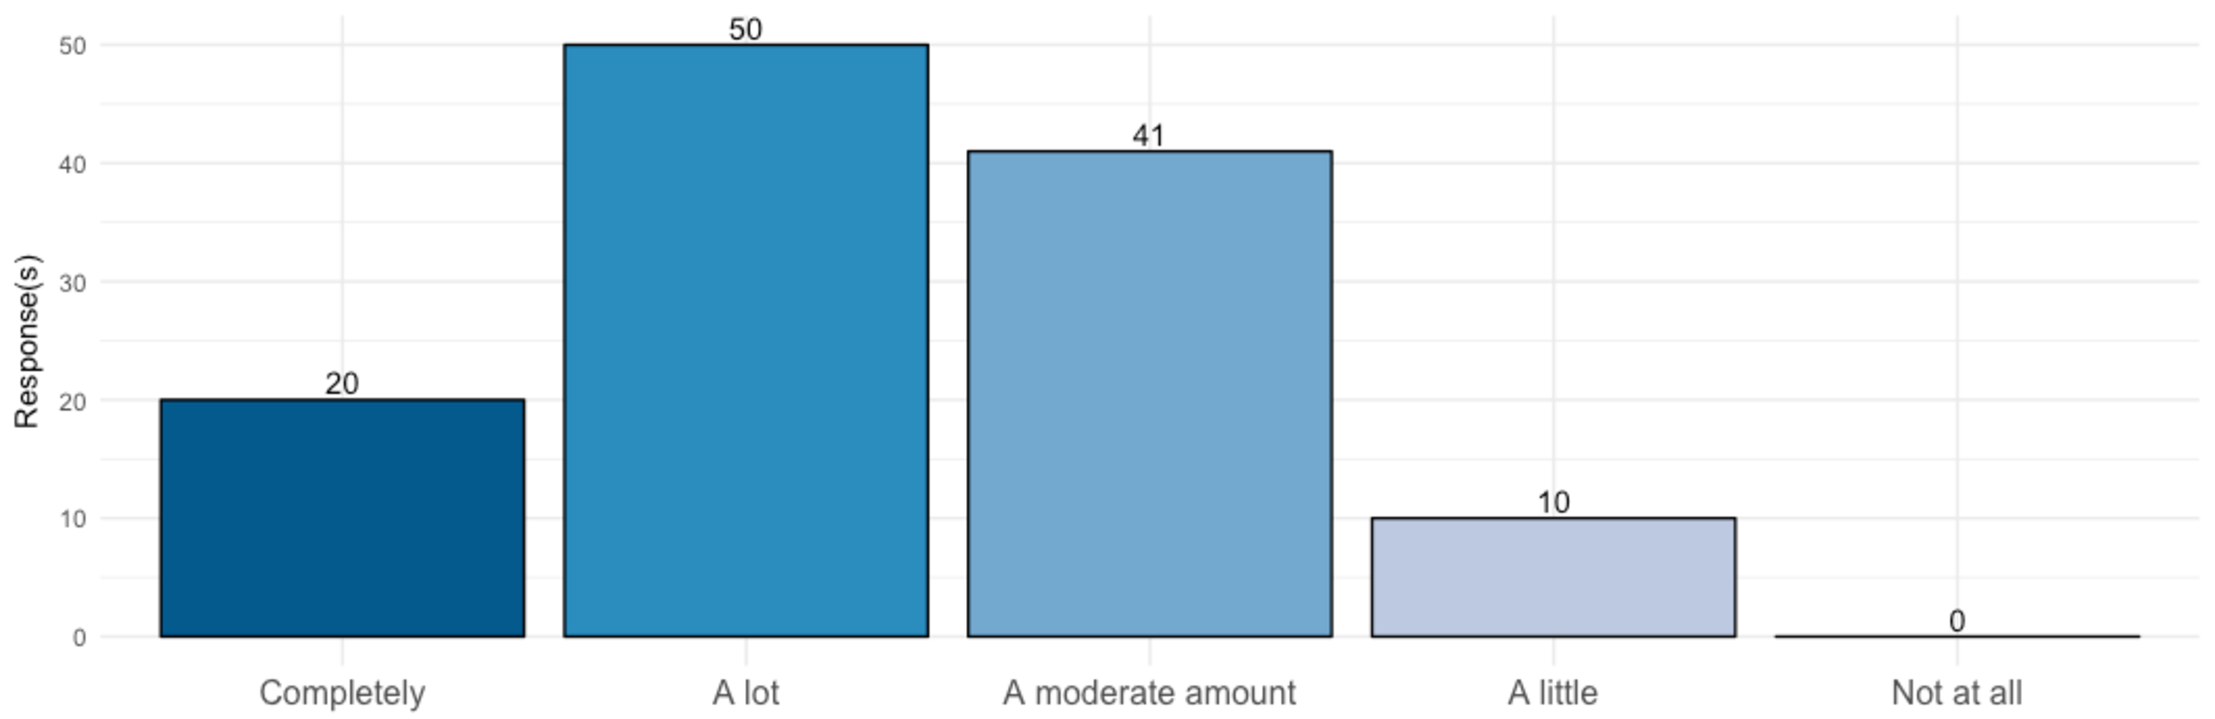
\includegraphics[width=0.95\textwidth,keepaspectratio]{s2_tool_trust}}
	\caption{Degree of Trust for Merging, History Exploration, and Conflict Resolution Tools. Scale: 1 is \textit{completely} and 5 is \textit{not at all}. 121 out of 162 respondents (74.69\%) provided a response to this question in the \textit{Barriers Survey}~(S2).\vspace*{-0.3\baselineskip}}
	\label{fig:tool_trust}
\end{figure}

Based upon this theme of mistrust, we asked S2 survey participants to rate the degree to which they trust their merging, history exploration, and conflict resolution tools.
We received 121 responses to this question, with a mean score of 3.66 placing the most common responses between \textit{a moderate amount} and \textit{a lot} of trust (Figure~\ref{fig:tool_trust}).
Assuming that responses of \textit{a moderate amount}, \textit{a little}, or \textit{not at all} indicate some degree of mistrust, we find that 42.15\% of developers experience some gap in toolset trust.

However, the severity of toolset mistrust is not as significant as our interview results suggested.
Only 8.26\% of developers indicated that they trust their toolset \textit{a little} or \textit{not at all} (10 out of 121 responses).
As the results of the survey were counter to our interview results, we looked further. We found that: (1) participants reported on the trust levels of the tools that they regularly use, and (2) a large number of participants reported that they had discontinued using toolsets when they ran into errors. This indicates that if participants had reported their trust level of these discontinued tools the results would have been lower.

\nsubsection{Perceptions of Tool Effectiveness}\label{tool_effectiveness}
The perceived size and complexity of merge conflicts affect the way in which developers plan, allocate, and enact resolutions.
To understand the degree to which these two factors impact developers' perceptions about the effectiveness of their toolsets, we asked survey participants to rate their toolset across four different merge conflict archetypes: (A1) \textit{simple, small merge conflicts}, (A2) \textit{simple, large merge conflicts}, (A3) \textit{complex, small merge conflicts}, and (A4) \textit{complex, large merge conflicts}.

\begin{figure*}[!htbp]
\centering
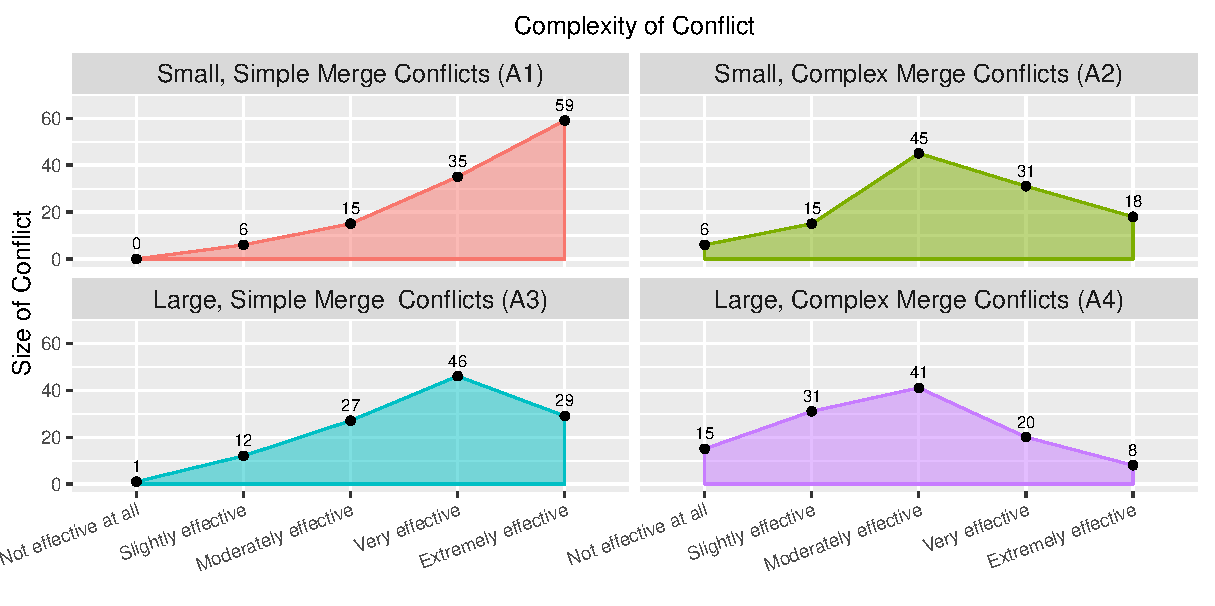
\includegraphics[width=1.01\textwidth]{ConflictComplexityVsSize.pdf}
\caption{Effectiveness of developers' toolsets in supporting perceived size and complexity of merge conflicts. Dot values indicate the number of S2 survey responses for effectiveness of a particular merge conflict size and complexity, and the vertical height of each segment indicating the number of responses at each degree of effectiveness.\vspace*{-0.3\baselineskip}}
\label{size_vs_complexity}
\end{figure*}

Since individual participants have different toolsets, and consider different factors when determining the perceived size and complexity of a merge conflict, we instructed participants to rate their own toolset against these archetypes using their notion of what constitutes a simple vs. complex and small vs. large merge conflict.
Fig.~\ref{size_vs_complexity} provides a visual illustration of the results of this survey question.

Observing the overall trends when moving between plots lines, we find that developers perceive complexity of the conflict to have a greater impact on the effectiveness of their merge toolsets than the size of merge conflicts.
Numerical analysis confirms this when finding that the mean response for archetype (A1) is 4.278 (where 5 is \textit{Extremely Effective} and 1 is \textit{Not effective at all}), (A2) is 3.782, (A3) is 3.347, and (A4) is 2.783.
The shift from \textit{small} to \textit{large} merge conflict size (A1 to A2) results in a difference in mean responses of 0.496, whereas the shift from \textit{simple} to \textit{complex} merge conflict complexity results in a difference in mean responses of 0.930.

These results suggest that merge tools are currently equipped to handle increases in the size of merge conflicts, but not as well equipped for increases in complexity.
The increasing amount of code being developed in distributed environments means that scaling support in both dimensions is necessary to accommodate developers' needs.